\documentclass[]{gshs_exam_T}

\usetikzlibrary{patterns,decorations.pathmorphing,arrows.meta,calc}
\usepackage{bm}

\usepackage{tikz-3dplot}


\makeatletter
\myyear{2018}\let\MyYear\@myyear %학년도
\semester{1}\let\Semester\@semester %학기
\exams{1차 지필평가}\let\Exams\@exams %1차,2차 지필평가
\subject{일반물리학I}\let\Subject\@subject %과목명
\credits{3} %학점
\pfscore{100} %만점
\examtime{60분} %시험시간
\examinerI{박지연} %출제1
\examinerII{정\hspace{1em}혁} %출제2
\examinerIII{한기덕}%출제3
\makeatother

%% 한글줄간격 %%
\renewcommand{\baselinestretch}{1.3}

\begin{document}

\maketitle

%%% page 1 %%%
\begin{multicols*}{2}
\noindent\fbox{\parbox{0.98\columnwidth}{\vspace*{-0.6em}
\begin{enumerate}[leftmargin=5.5mm,label=※]
\item 문항에 따라 배점이 다르므로 각 물음의 끝에 표시된 배점을 참고하시오.\\[-2.2em]
\item 서술형 ( 100 )점
\end{enumerate}\vspace{-0.6em}}}\vspace{1em}

\begin{questions}
\extrawidth{8.1em}
%%% Problem 1 %%%
\addpoints
\question 그림은 질량이 $2m$인 물체 B 위에 질량이 $m$인 물체 A가 놓여있고, 용수철 상수가 $k$인 용수철 2개와 B가 연결되어 수평면 위에서 평형을 이루고 있는 모습을 나타낸 것이다. A와 B 사이의 정지마찰계수는 $\mu$이고, B와 수평면 사이에 마찰은 없다. (단, 중력가속도는 $g$이다.)\droptotalpoints
\begin{center}
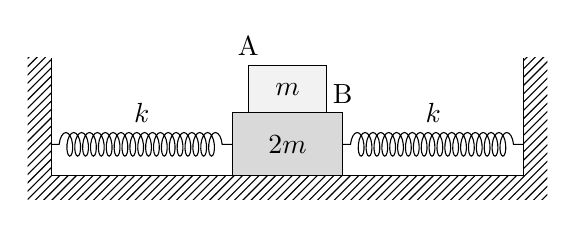
\begin{tikzpicture}
\fill[pattern=north east lines] (-0.3,-0.3) rectangle (6.3,1.5);
\fill[white] (0,0) rectangle (6,1.6);
\draw (0,1.5) -- (0,0) -- (6,0) -- (6,1.5);
\draw[fill=black!15] (2.3,0) rectangle (3.7,0.8) node[pos=0.5]{$2m$};
\node[above] at (3.7,0.8) {B};
\draw[fill=black!5] (2.5,0.8) rectangle (3.5,1.4) node[pos=0.5]{$m$};
\node[above] at (2.5,1.4) {A};
\draw[decorate,decoration={coil,aspect=0.4,amplitude=1.5mm,segment length=1mm,pre length=1mm,post length=0.6mm}] (0,0.4) -- (2.3,0.4) node[pos=0.5,above=1.5mm]{$k$};
\draw[decorate,decoration={coil,aspect=0.4,amplitude=1.5mm,segment length=1mm,pre length=1mm,post length=0.6mm}] (3.7,0.4) -- (6,0.4) node[pos=0.5,above=1.5mm]{$k$};
\end{tikzpicture}
\end{center}
\begin{parts}
\part[5] \ssh\ A와 B가 붙어있는 상태로 단순조화운동을 할 때, 각각의 운동 방정식을 세워 진동의 주기를 구하시오.\droppoints
\vspace{15em}
\part[6] \ssh\ 운동하는 B 위에서 A가 미끄러지기 위한 B의 최소 진폭을 구하시오.\droppoints

\vspace*{\fill}
\columnbreak
\vspace*{-0.8em}
\part[3] \ssh\ A와 B가 붙어있는 상태로 액체 속에 완전히 잠겨서 감쇠진동을 한다. 이때 작용하는 감쇠력 $F_d =-bv$이다. 감쇠력이 있을 때의 각진동수는 감쇠력이 없을 때와는 다르게 나타난다. 감쇠력의 유무에 따른 각진동수 차이를 구하시오. (단, A, B의 밀도는 액체의 밀도보다 크며, $x\ll 1$일 때 $(1+x)^n \approx 1+nx$이고, $b^2 \ll km$이다.)\droppoints
\end{parts}

\end{questions}
\end{multicols*}

%%% page 2 %%%

\begin{multicols*}{2}
\begin{questions}\extrawidth{8.1em}\setcounter{question}{1} %이전 페이지 마지막 문항 번호 입력

%%% Problem 2 %%%
\addpoints
\question 그림은 질량 $m$인 위성이 질량 $M$인 행성을 초점으로 하는 타원궤도를 따라 돌다가 점 P에서 추진력에 의해 순간적으로 속력이 증가하여 행성을 중심으로 원궤도를 따라 운동하고 있는 모습을 나타낸 것이다. 점 P, Q는 각각 타원궤도의 원일점과 근일점이고, P에서 타원궤도와 원궤도가 접한다. 점 P, Q, R은 동일 직선상에 있으며, 행성의 중심으로부터 P까지의 거리는 $3l$이다. (단, 위성에는 행성에 의한 중력만 작용하고, $m\ll M$이며, 중력상수는 $G$이다.)\droptotalpoints
\begin{center}
\begin{tikzpicture}
\def\a{2}
\def\b{1.5}
\def\c{sqrt(\a*\a-\b*\b)}
\coordinate (O) at (0,0);
\coordinate (P) at ({-\a-\c},0);
\coordinate (Q) at ({\a-\c},0);
\coordinate (R) at ({\a+\c},0);
\coordinate (st) at ({(\a+\c)*cos(140)},{(\a+\c)*sin(140)});
\draw[densely dashed,thick,domain=0:360,samples=37,smooth] plot ({\a*cos(\x)-\c},{\b*sin(\x)});
\draw[densely dashed,thick] (O) circle ({\a+\c});
\draw (P) -- (R);
\fill[black] (P) circle (0.06) node[left]{P};
\fill[black] (Q) circle (0.06) node[anchor=north west]{Q};
\fill[black] (R) circle (0.06) node[right]{R};
\draw[-latex,very thick] (st) arc (140:100:{\a+\c});
\draw[ball color=black!30] (O) circle (0.2) node[below=0.2cm]{\small 행성};
\draw[ball color=black!30] (st) circle (0.1) node[anchor=south east]{\small 위성};
\draw (O) to[out=150,in=30] (P); 
\node[above=0.5cm] at ($(O)!0.5!(P)$) {$3l$};
\node[above=0.2cm] at (O) {$M$};
\node[anchor=north west] at (st) {$m$};
\end{tikzpicture}
\end{center}
\vspace{0.3em}
\begin{parts}
\part[5] \ssh\ 타원궤도, 원궤도를 따라 운동하는 위성의 주기가 각각 $2\sqrt{2}T$, $3\sqrt{3}T$일 때, Q에서 R까지의 거리를 구하시오.\par\droppoints
\vspace{15em}
\part[6] \ssh\ 타원궤도에서 원궤도로 진입할 때, 추진력이 한 일과 행성의 중력이 위성에게 한 일을 구하시오.\droppoints

\vspace*{\fill}
\columnbreak

\part[7] \ssh\ 타원궤도, 원궤도를 따라 운동하는 위성이 P를 지나는 순간의 속력을 각각 $v_e$, $v_c$라 할 때, $v_c /v_e$를 구하시오.\par\droppoints
\end{parts}

\vspace{20em}

%%% problem 3 %%%
\addpoints
\question 그림은 선밀도 $\mu$, 길이 $L$의 팽팽한 줄에 질량 $m$인 물체와 진동자가 연결된 것을 나타낸 것이다. 점 P를 통해 $y=y_m \sin(\tfrac{4\pi}{L}x-2\pi at)$ ($a$는 상수)의 파동이 만들어지고, 고정된 점 Q에서 파동이 반사된다. 점 P와 Q에서의 진폭은 미미하므로 각각 마디로 볼 수 있다. (단, 중력가속도는 $g$이다.)\droptotalpoints
\begin{center}
\begin{tikzpicture}
\draw[fill=black!5] (0,-0.4) rectangle (1.1,0.4) node[pos=0.5]{\small 진동자};
\draw[thick] (1.1,0) -- (6,0) arc (90:0:0.06) -- (6.06,-1);
\fill[black] (1.4,0) circle (0.06) node[above=0.06]{P};
\fill[black] (6,-0.06) circle (0.06) node[above=0.06]{Q};
\draw[thin] (1.4,0) -- (1.4,-0.5);
\draw[thin] (6,-0.06) -- (6,-0.5);
\draw[latex-latex] (1.4,-0.3) -- (6,-0.3) node[fill=white,pos=0.5]{$L$};
\draw[fill=black!15] ({6.06-0.5},-1) rectangle ({6.05+0.5},-2) node[pos=0.5] {$m$};
\end{tikzpicture}
\end{center}
\begin{parts}
\part[4] \ssh\ $a$를 주어진 문자로 나타내시오.\droppoints
\vspace{6em}
\part[4] \ssh\ 줄에서 정지파가 만들어지는지 그렇지 않은지 그 이유와 함께 설명하시오.\droppoints
\vspace{6em}
\part[3] \ssh\ 진동수를 유지한 상태에서 줄에 연결된 물체의 질량을 $4m$으로 바꿨다. 이 때 만들어진 정지파의 조화차수를 구하시오.\droppoints
\end{parts}

\end{questions}
\end{multicols*}



\end{document}